\documentclass[10pt]{standalone}

\usepackage{pgf,tikz}
\usepackage{mathrsfs}
\usetikzlibrary{arrows}
\pagestyle{empty}
\begin{document}
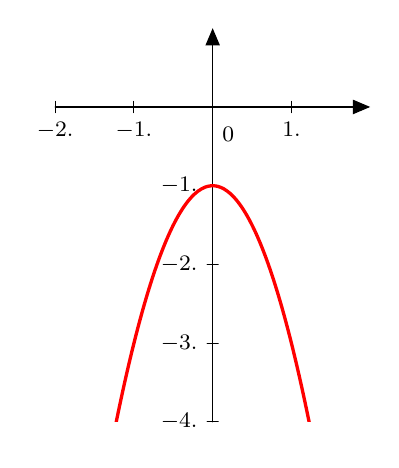
\begin{tikzpicture}[line cap=round,line join=round,>=triangle 45,x=1.0cm,y=1.0cm]
\draw[->,color=black] (-2.,0.) -- (2.,0.);
\foreach \x in {-2.,-1.,1.}
\draw[shift={(\x,0)},color=black] (0pt,2pt) -- (0pt,-2pt) node[below] {\footnotesize $\x$};
\draw[->,color=black] (0.,-4.) -- (0.,1.);
\foreach \y in {-4.,-3.,-2.,-1.}
\draw[shift={(0,\y)},color=black] (2pt,0pt) -- (-2pt,0pt) node[left] {\footnotesize $\y$};
\draw[color=black] (0pt,-10pt) node[right] {\footnotesize $0$};
\clip(-2.,-4.) rectangle (2.,1.);
\draw[line width=1.2pt,color=red,smooth,samples=100,domain=-2.0:2.0] plot(\x,{0-2.0*(\x)^(2.0)-1.0});
\end{tikzpicture}
\end{document}